\section{Experimenting with Reaching}

\subsection{Creating a Policy}
The next step was to create a policy network. As I am mainly working on imitation learning -and specifically behavioural cloning- from demonstrations provided by the system, my network needs to be able to ingest these demonstrations and generate actions in the action space of the robot. Following the earlier parameters of a demo, I created the following network, Figure \ref{fig:policy-arch}. This takes in the given wrist rgb image and extracts features, which are then interpreted into a $8$ dim vector of \textbf{float}s as an action. First $7$ corresponding to the $7$ joints of the \emph{Panda} robot, and holding a velocity value for them, while the final value is the gripper state, $0$ meaning closed and $1$ meaning open, which is clamped by the movement system under the hood.

\begin{figure}[h]
  \centering
  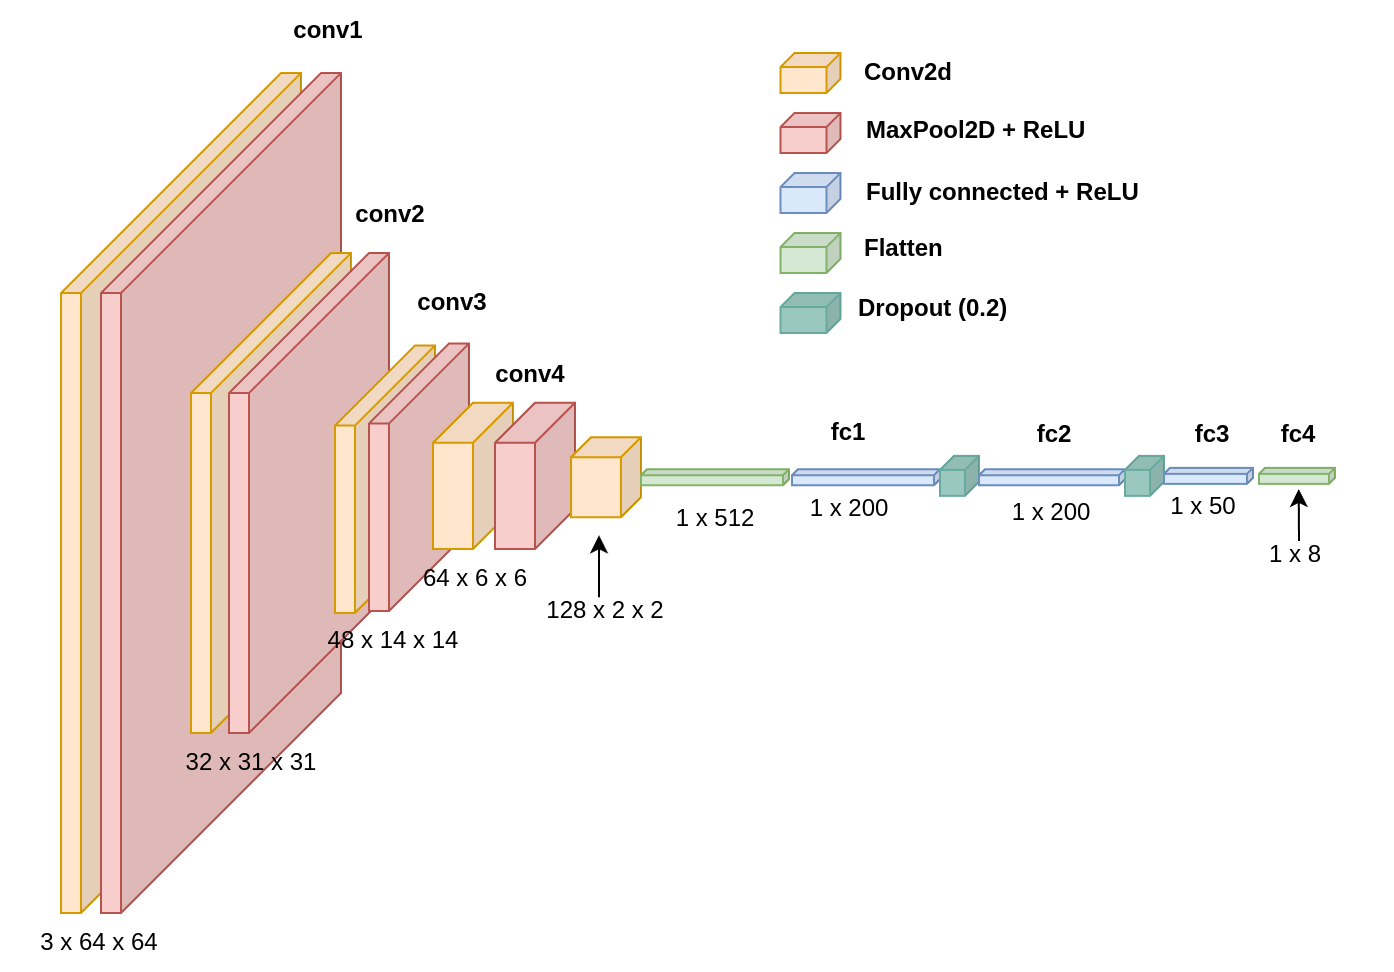
\includegraphics[width=0.6\textwidth]{assets/early-work/cnn-encoder-policy-head.png}
  \caption{Simple Policy Network Architecture}\label{fig:policy-arch}
\end{figure}\todo[color=blue]{ius the quality bad? reuload or reexport the xmml is in assets}

Along with the policy the second most important of any ML workload is the way the data us regularised, processed, and loaded into the system for training or testing.

\subsubsection{Data Processing}\todo{talk about rgb transforms? uniforming etc, or remove not sure}

\subsubsection{Data Loading}
I followed a simple flattening approach for loading the data into the system. Using PyTorch's \textbf{Dataset} and \textbf{DataLoader} classes I created a dataset that can take in a raw list of demonstration, then flattens its observations into a tensor of shape \(\langle 3,~64,~64 \rangle \) (permuted from the usual \(\langle 64,~64,~3 \rangle \) for images due to Torch conventions of convolutional networks and where they expect the channel  dimension). Then the dataset makes individual observation indexable along with their corresponding action labels. Types given as:\mintinline{python}|DemoObsDataset: tensor[tensor[3,  64, 64], tensor[8]]|. Then the loader can manage the shuffling and batching as usual. Initially I kept the data unshuffled, to keep the data in its sequential form. While keeping the batch size as the demo length. This is because currently I am trying to overfit the network to the single demonstration given to it to gauge how long to train my networks for

\subsection{Initial Observations}
Starting with the 3 static versions of the task, where the target is placed as shown in \ref{fig:no-obs-3-views} seen from the wrist cameras. I wanted to get an idea of how to tune the policy parameters. While understanding the relationship between training length and varying observability of the target.

\begin{figure}[htbp]
  \begin{subfigure}{0.3\linewidth}
    \centering
    
\includegraphics[scale=0.4]{../fyp/assets/demo-trials-no_obs/tasks/static-tasks-camera/initial-obs-side_l.png}      
    \caption{Left Side}
  \end{subfigure}
  \hfill
  \begin{subfigure}{0.3\textwidth}
    \centering
    
\includegraphics[scale=0.4]{../fyp/assets/demo-trials-no_obs/tasks/static-tasks-camera/initial-obs-central.png}
    \caption{Central}
  \end{subfigure}
  \hfill
  \begin{subfigure}{0.3\linewidth}
    \centering
    
\includegraphics[scale=0.4]{../fyp/assets/demo-trials-no_obs/tasks/static-tasks-camera/initial-obs-side_r.png}
    \caption{Right Side}
  \end{subfigure}%
  \caption{Three variations of the reach task with the obstacles sometimes out of view}\label{fig:no-obs-3-views}
\end{figure}

I tested multiple epochs of training with the simple policy and recorded the final distance to the target at the end of their episode. The episode length is determined by the demo lengths, which I defaulted to the maximum, will also try mean, as keeping a static episode length doesn't make sense (especially on later tasks where the demonstration episodes can drastically vary in length)

The success of the tasks are wired to reaching the target in the simulator and will send a \emph{DONE} signal if it is reached. This happens around $0.12$ metres to the target. I have also observed the target will reach a very close distance but it won't trigger the detection in Coppelia, I think this must be a bounding box issue, wither the dummy objects that are doing the collision detection are missing each other, or the polling rate in the simulator is not frequent enough to detect this change. Either way, I added a way to count closeness into success if it were close enough.

\subsubsection{Static Tasks}
Testing on the static versions of the task, a simple policy with training around $20$ to $100$ epochs seems to do the job well, see Figure \ref{fig:rno-static}. And this is mostly because without variation in position simple Behavioural Cloning can be employed by overfitting to the data given. 

As I trained for longer it seemed to overfit early move really slowly at the start of the episode, wasting steps and ending up far from the target. Curious observation is \todo[color=purple]{} the central tasks behaves better at higher epochs which I believe is not necessarily because of visibility (the \emph{conv} features are not necessarily guiding anything with $1$ demo) but rather the centrality, as it is right above the gripper a simple downward bias allows the arm to easily get close to the target.

\begin{figure}[htpb] % htpb allows all placement
  \centering
  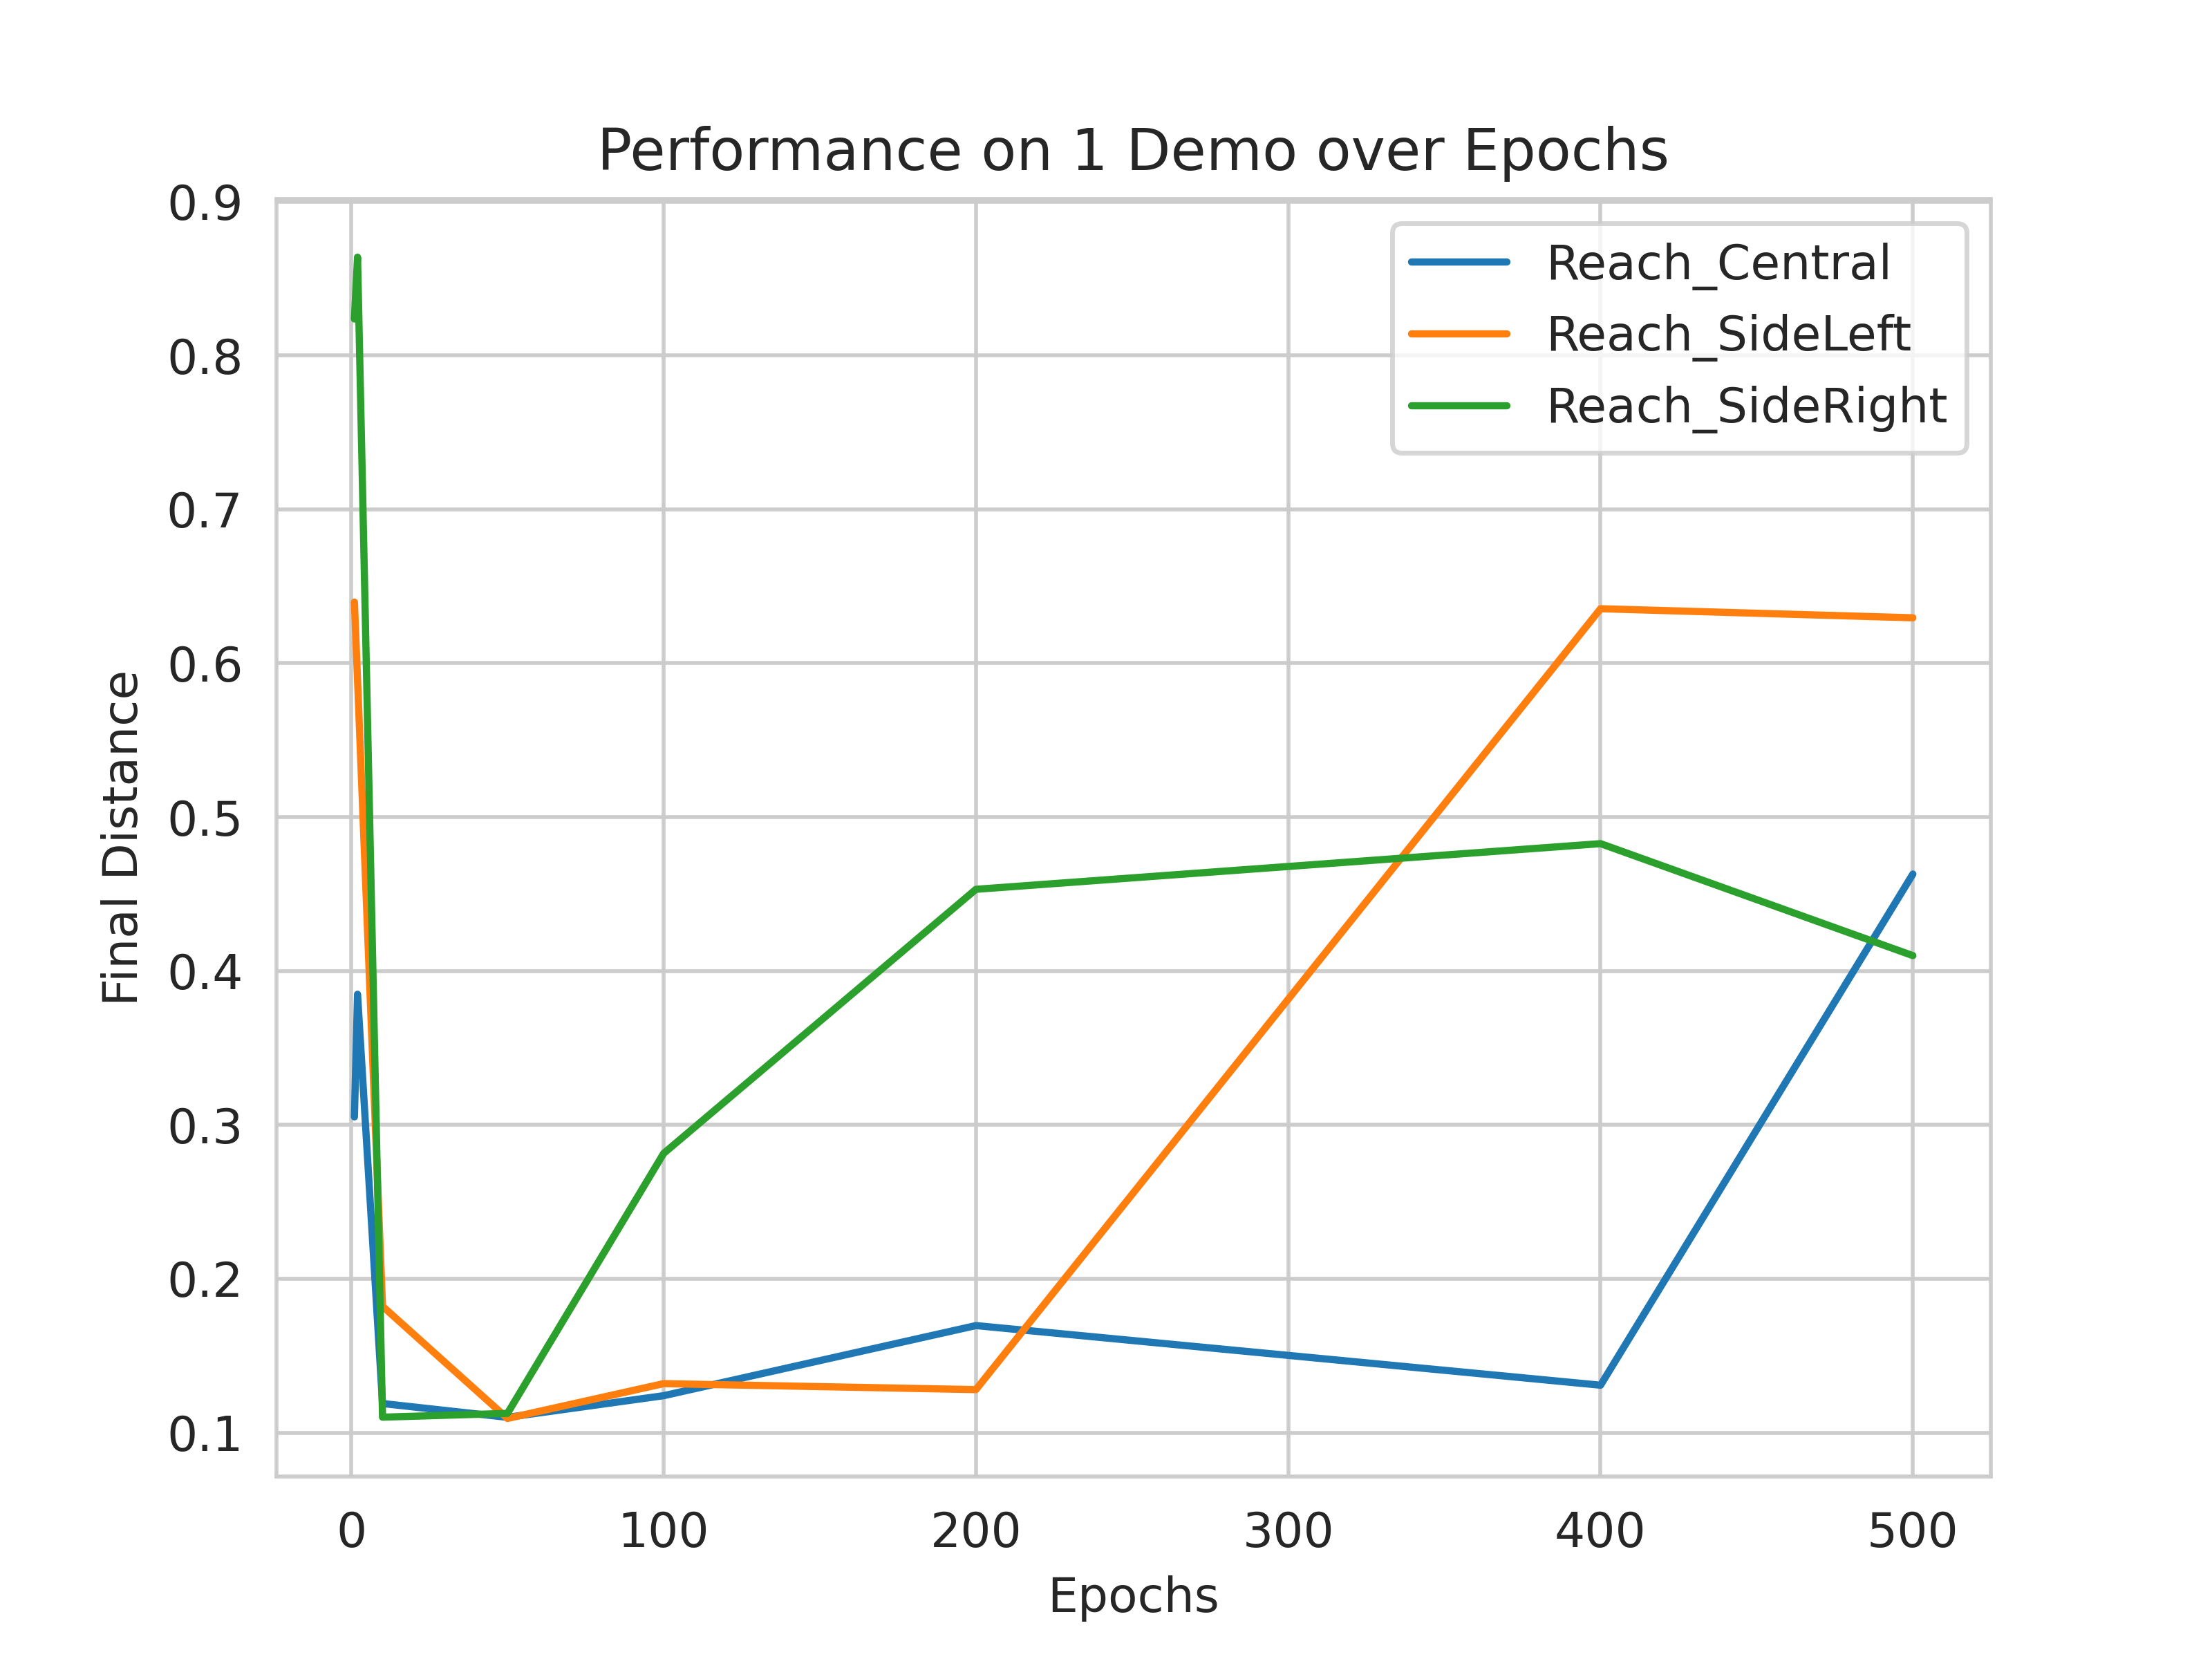
\includegraphics[scale=0.5]{assets/cam-comb/reach-no-obs/rno_static.png}
  \caption{Epoch experiments with the static tasks using a single demonstration}\label{fig:rno-static}
\end{figure}

\subsubsection{Placing Randomly}
To test generalisability, I created a dynamic version of the task, where the target is now randomly placed within view (not necessarily always fully within view, but at least some parts are visible). This is achieved by using a \verb|SpawnBoundary| and randomly sampling the location of the target withing this for every new variation of the task, or for every new episode. Which can be seen in Figure \ref{fig:reach-no-obs}, the white dotted box being the boundary. This boundary is not rendered in the simulation visually. This guarantees variety in demonstrations as well as helps us create a generalisable policy.

\begin{figure}[htpb] % htpb allows all placement
  \begin{subfigure}{0.50\linewidth}
    \centering
    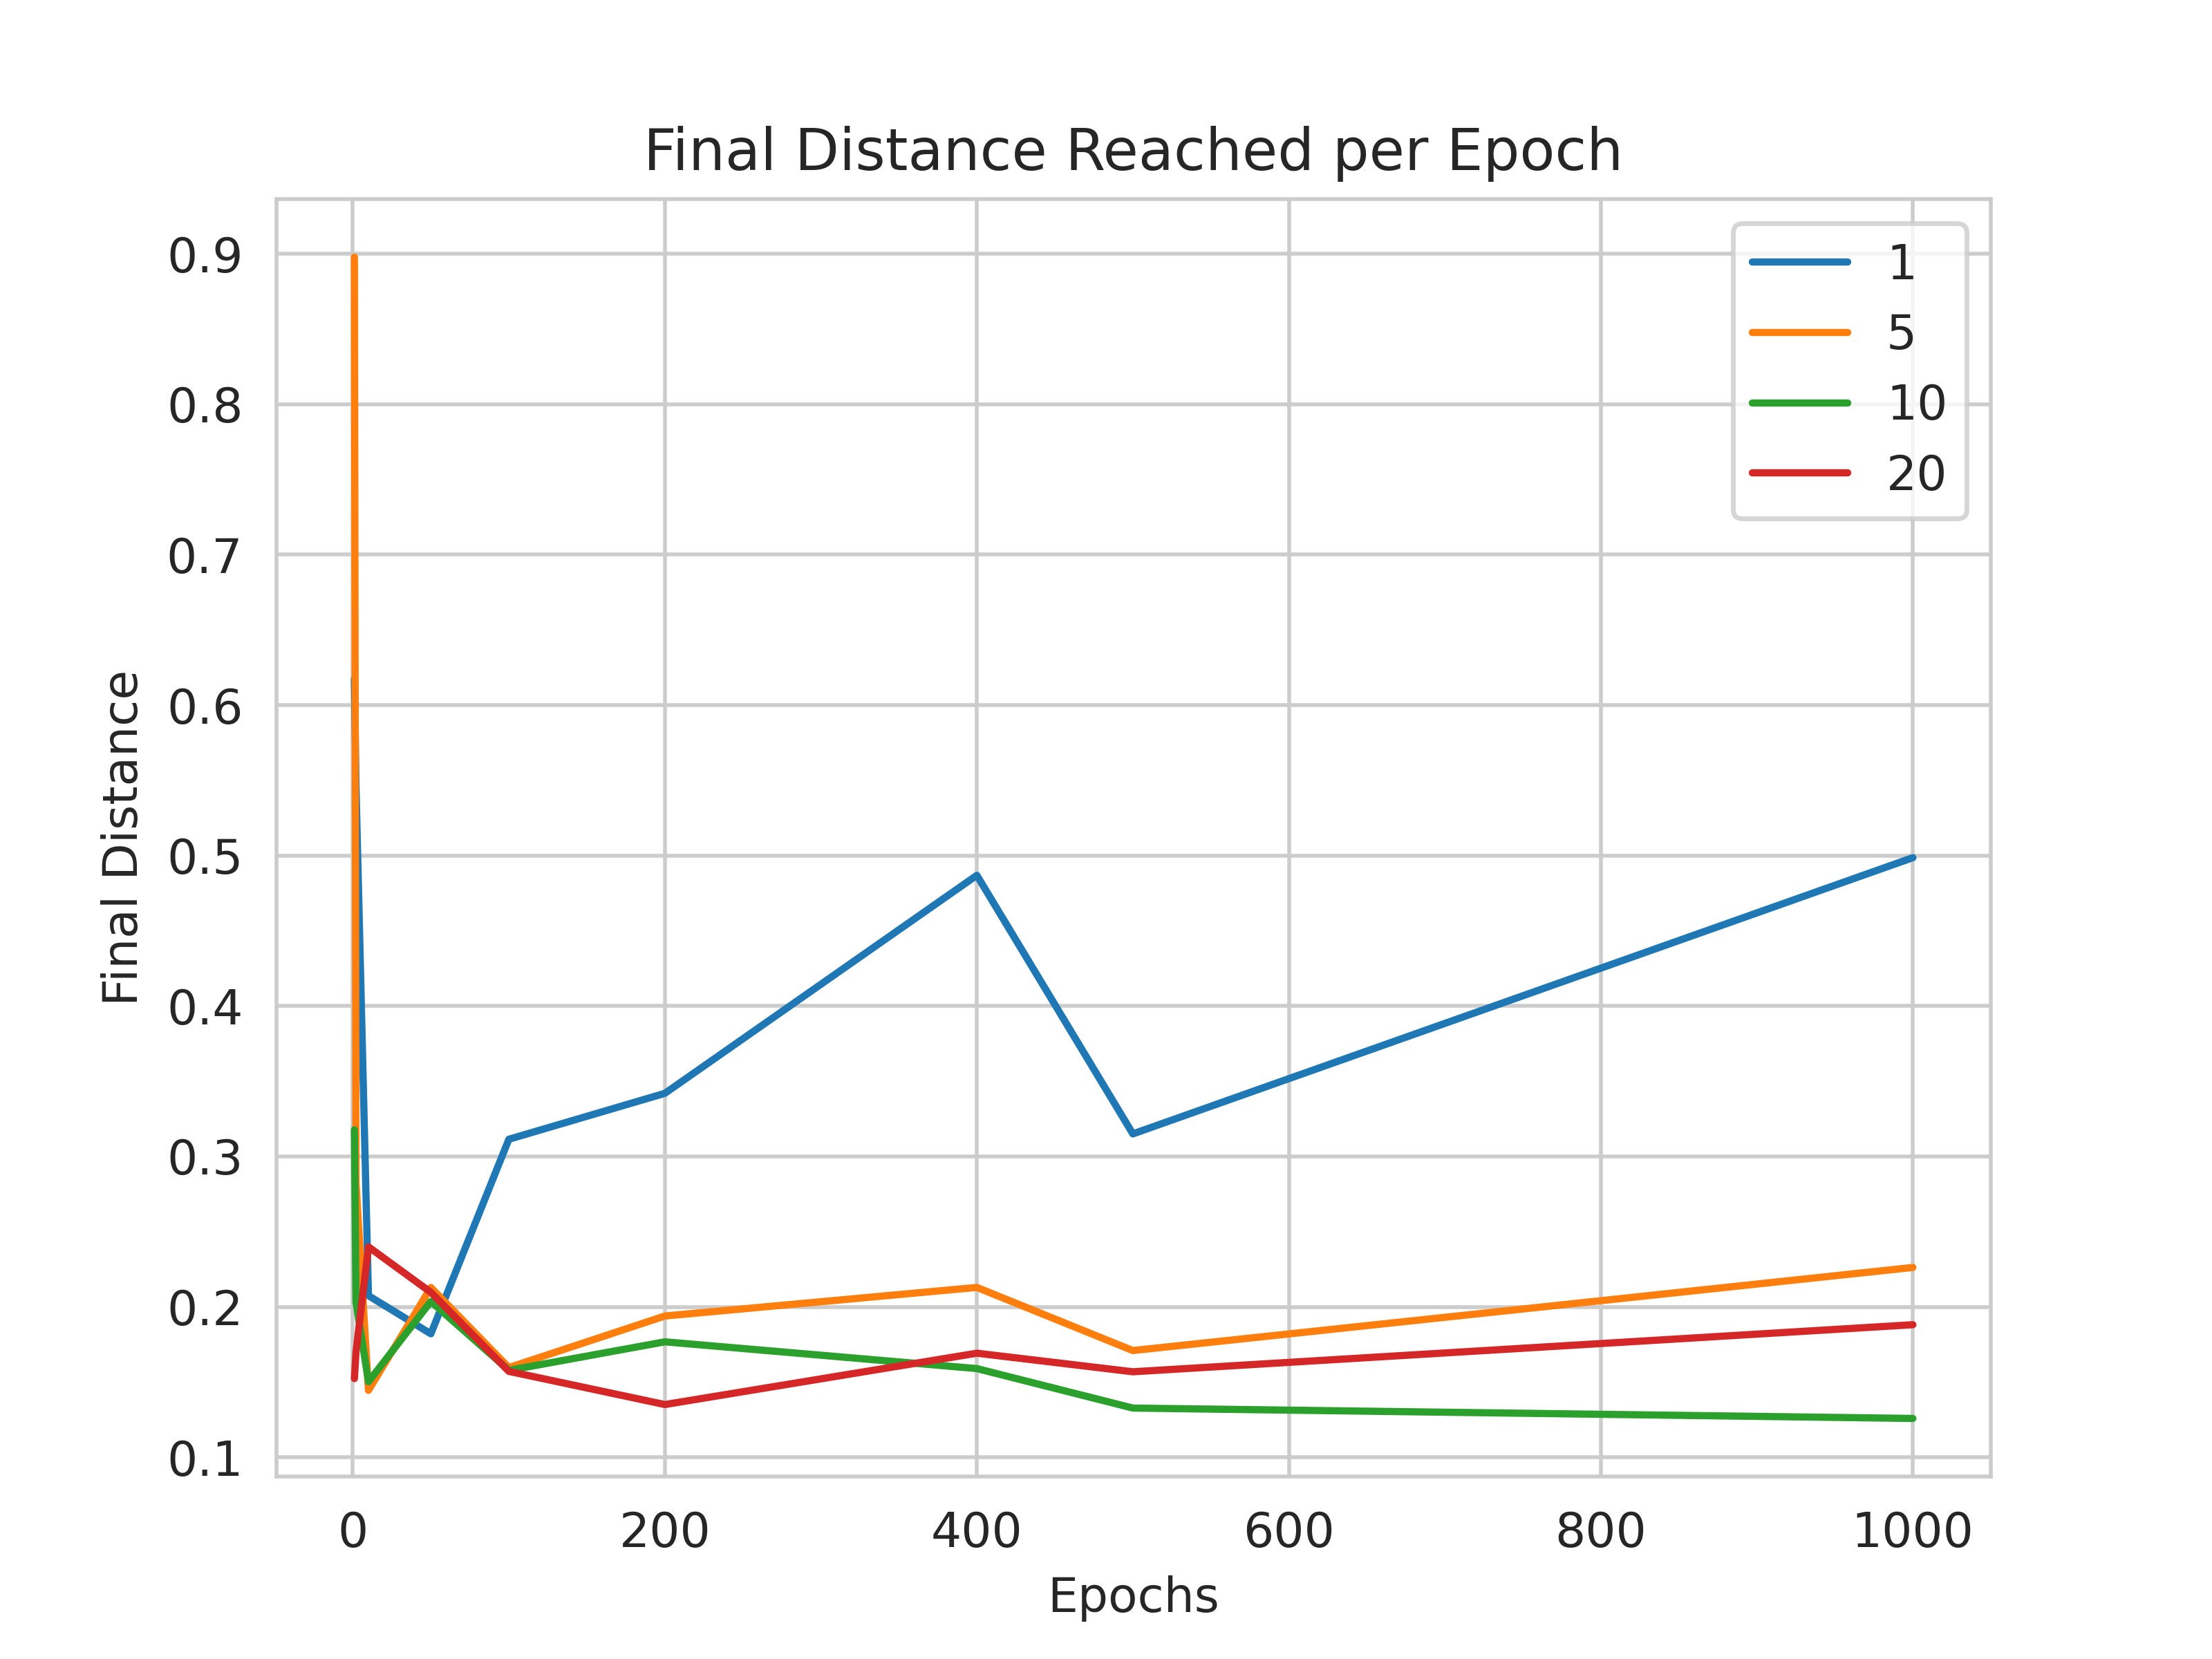
\includegraphics[width=\linewidth]{assets/cam-comb/reach-no-obs/rno_random-dist.png}
    \caption{Average Final Distance to Target}\label{subfig:rno-random-dist}
  \end{subfigure}
  \hfill
  \begin{subfigure}{0.50\linewidth}
    \centering
    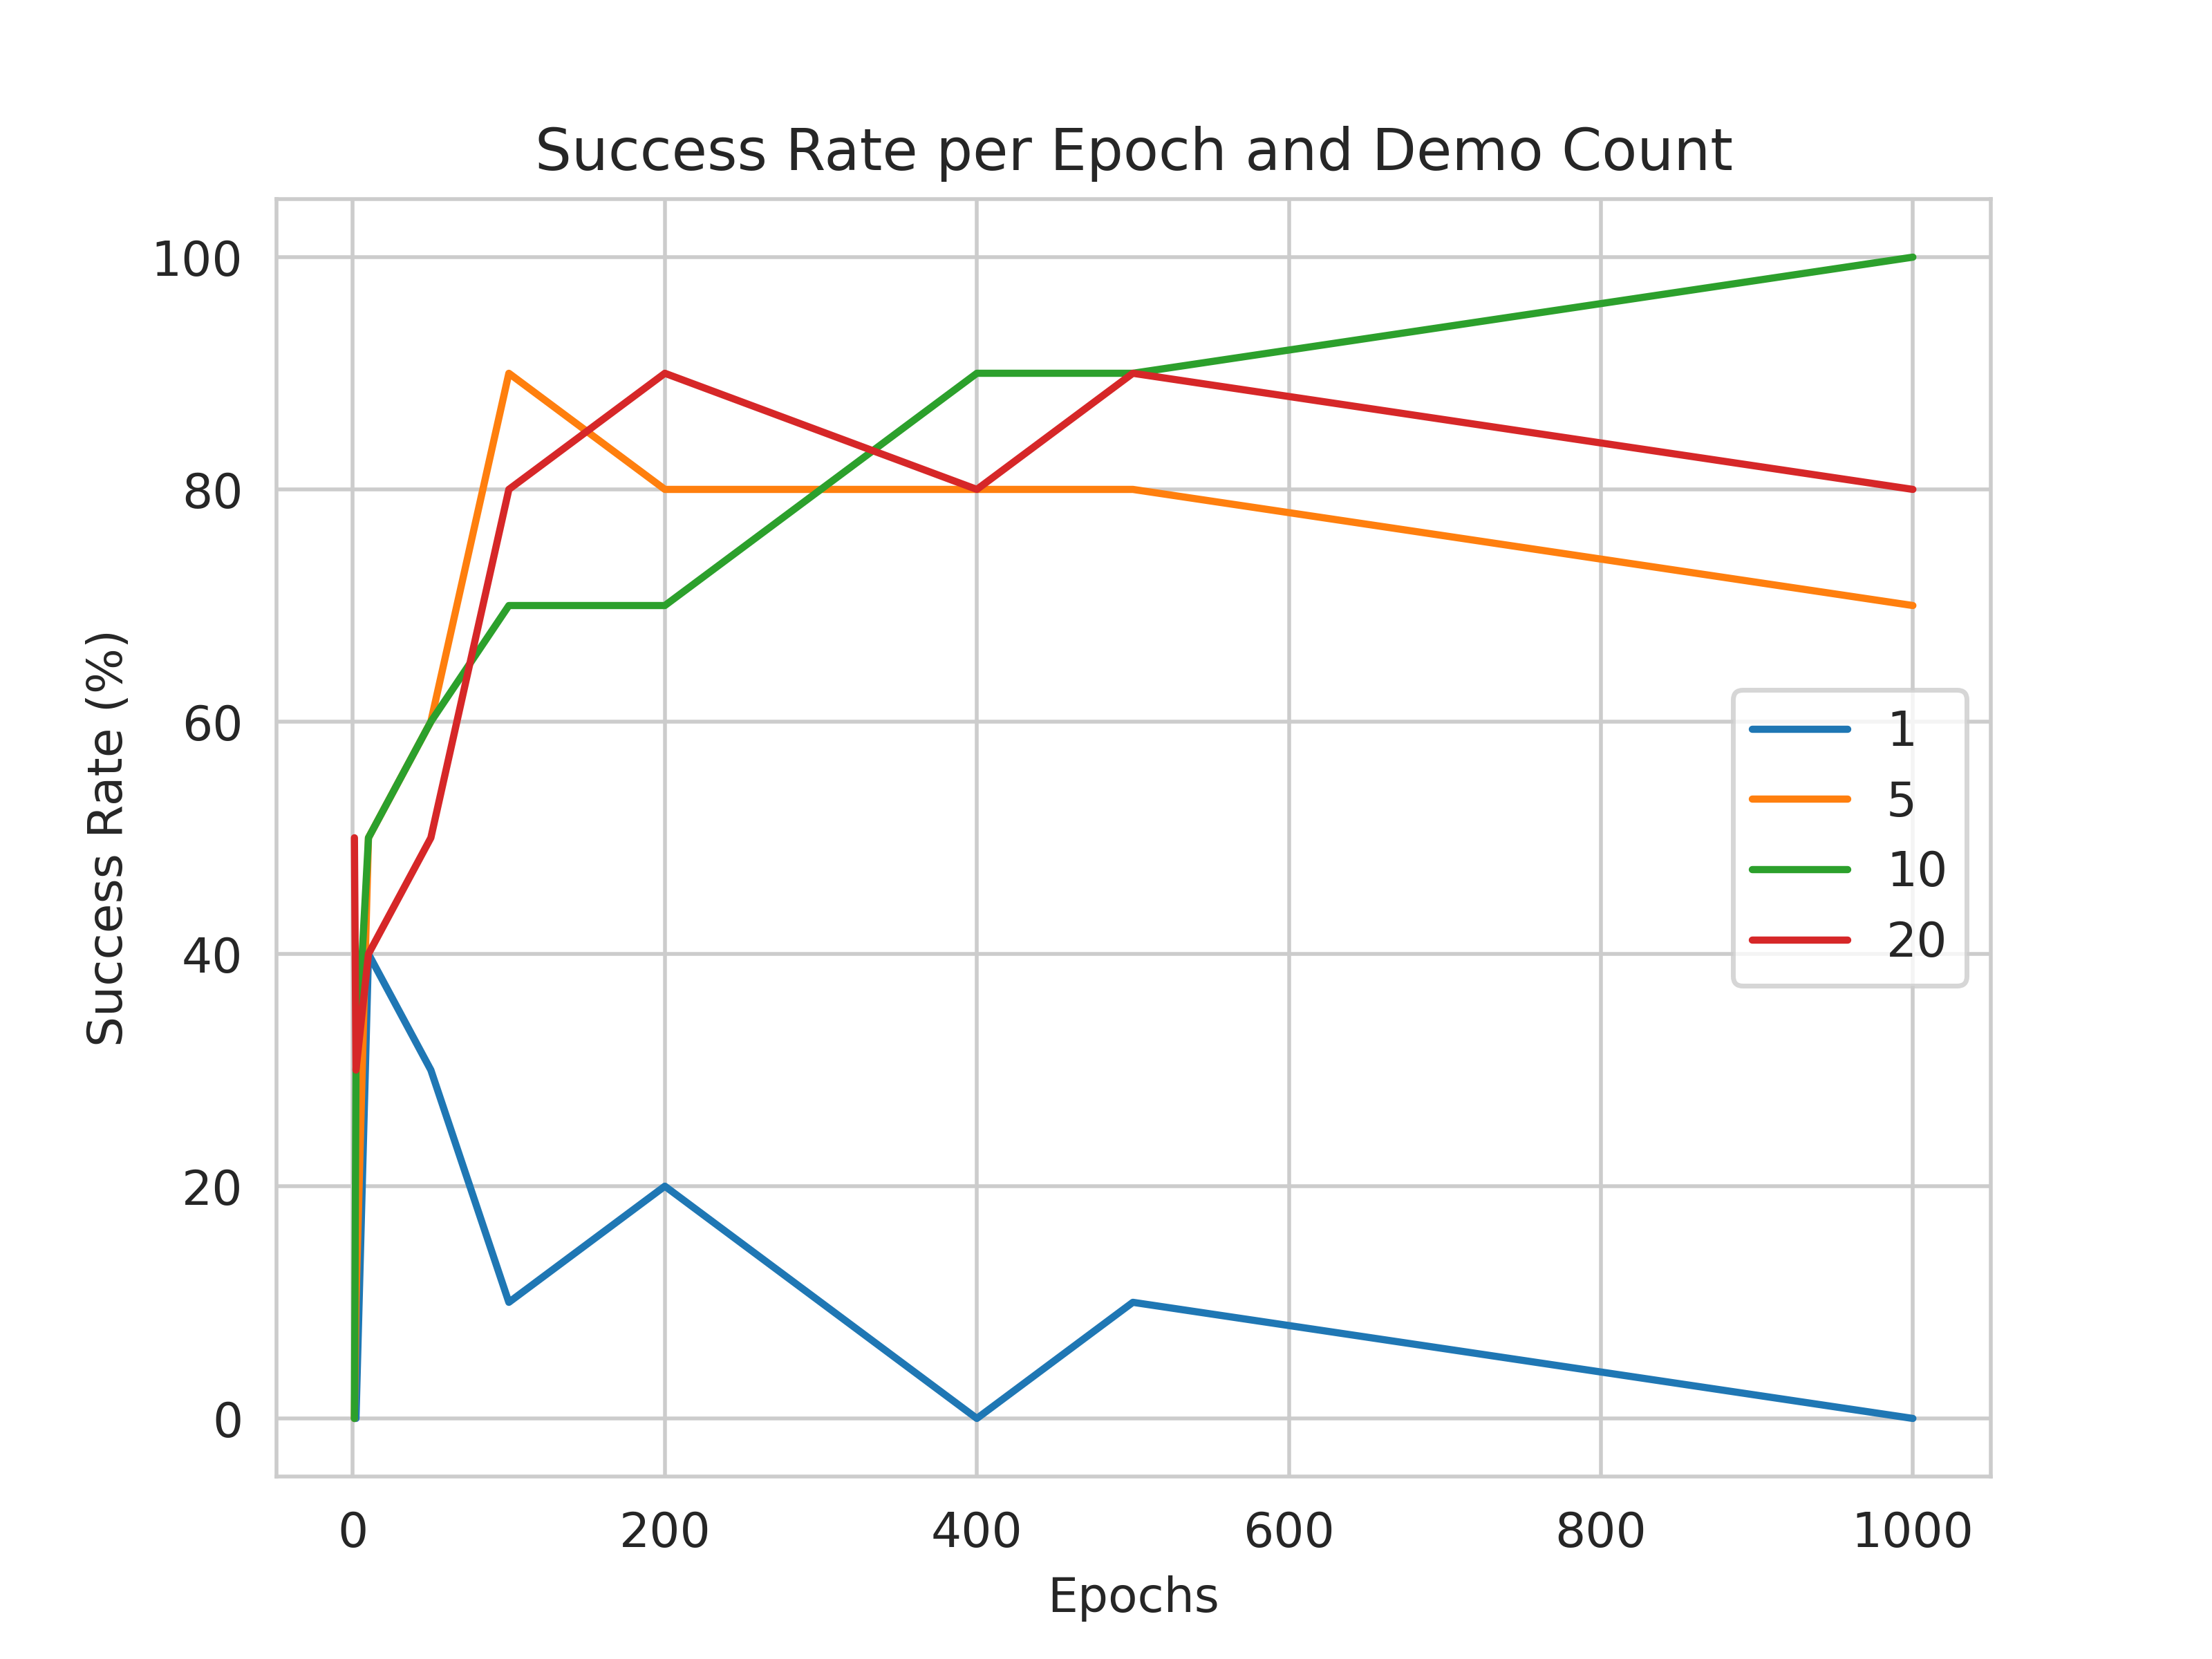
\includegraphics[width=\linewidth]{assets/cam-comb/reach-no-obs/rno_random-success.png}
    \caption{Success Rate (\%) for the $10$ Test Demos}\label{subfig:rno-random-success}
  \end{subfigure}
  \caption{Experiments with randomly placed target}\label{fig:rno-random}
\end{figure}

To run the random tests, shown in Figure \ref{fig:rno-random}, in a comparable manner I reused my set of demos that were created and saved earlier for this task for training. Then a set of 10 demos were randomly generated at the start and after the agent with the specific parameters were trained, I evaluated these policies against the test counterparts.

Looking at graph \ref{subfig:rno-random-dist}, we can see that providing more demonstrations helps the policy generalise better to random locations, where the sweet spots seems to be around 10 demos and around $500$ where the success rate (\ref{subfig:rno-random-success}) is quite high

\subsection{Camera Limitations}\todo[color=red]{reread and make sure it is a good starter segue to obs (maybe move these to after obs?), mention this under reachObs! MOVE}
I started this section by limiting the learning to only the wrist mounted camera, which works well for this specific unobscured task. Introducing some of the other RGB cameras, specifically the \verb|left shoulder| or the \verb|right shoulder| views, does not necessarily benefit the performance, see \ref{fig:rno-random-cams}. Conversely, we are increasing the training time by adding more channels to the convolutional layers, which can be considered a drawback.

\begin{figure}[htpb] % htpb allows all placement
  \begin{subfigure}{0.50\linewidth}
    \centering
    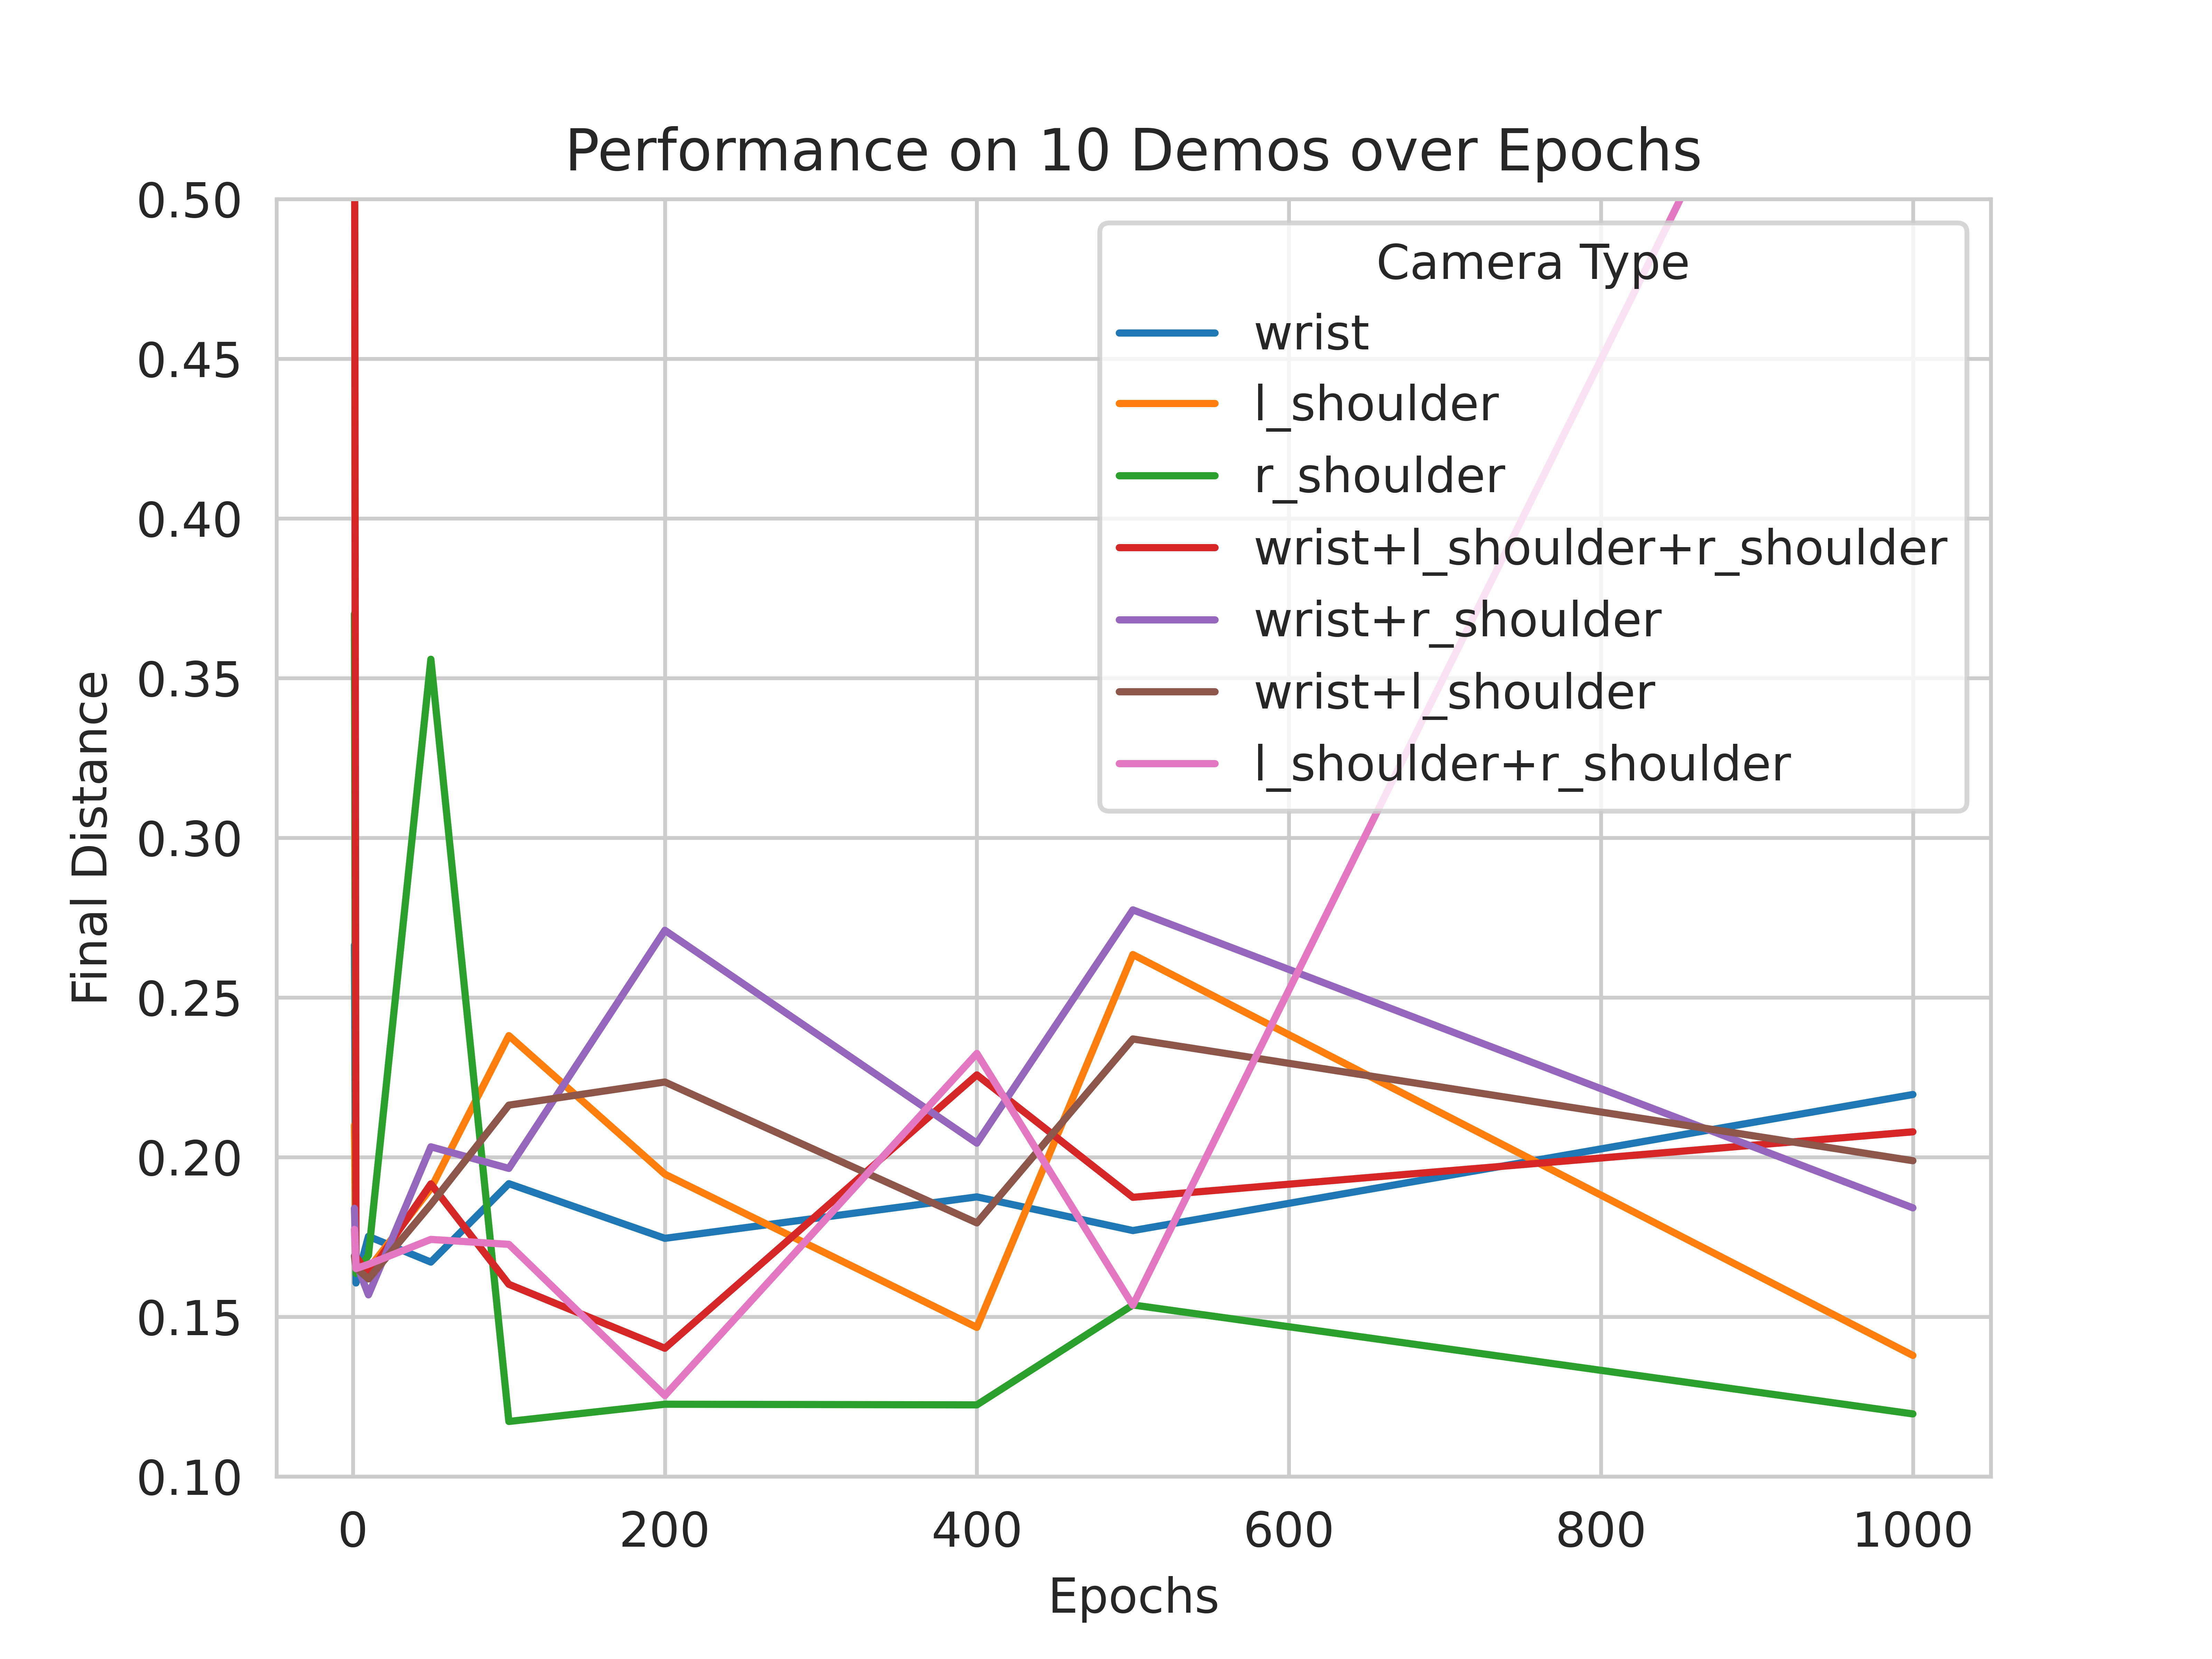
\includegraphics[width=\linewidth]{assets/cam-comb/reach-no-obs/rno_random-cams.png}
    \caption{Average Final Distance to Target}\label{subfig:rno-random-cams-dist}
  \end{subfigure}
  \hfill
  \begin{subfigure}{0.50\linewidth}
    \centering
    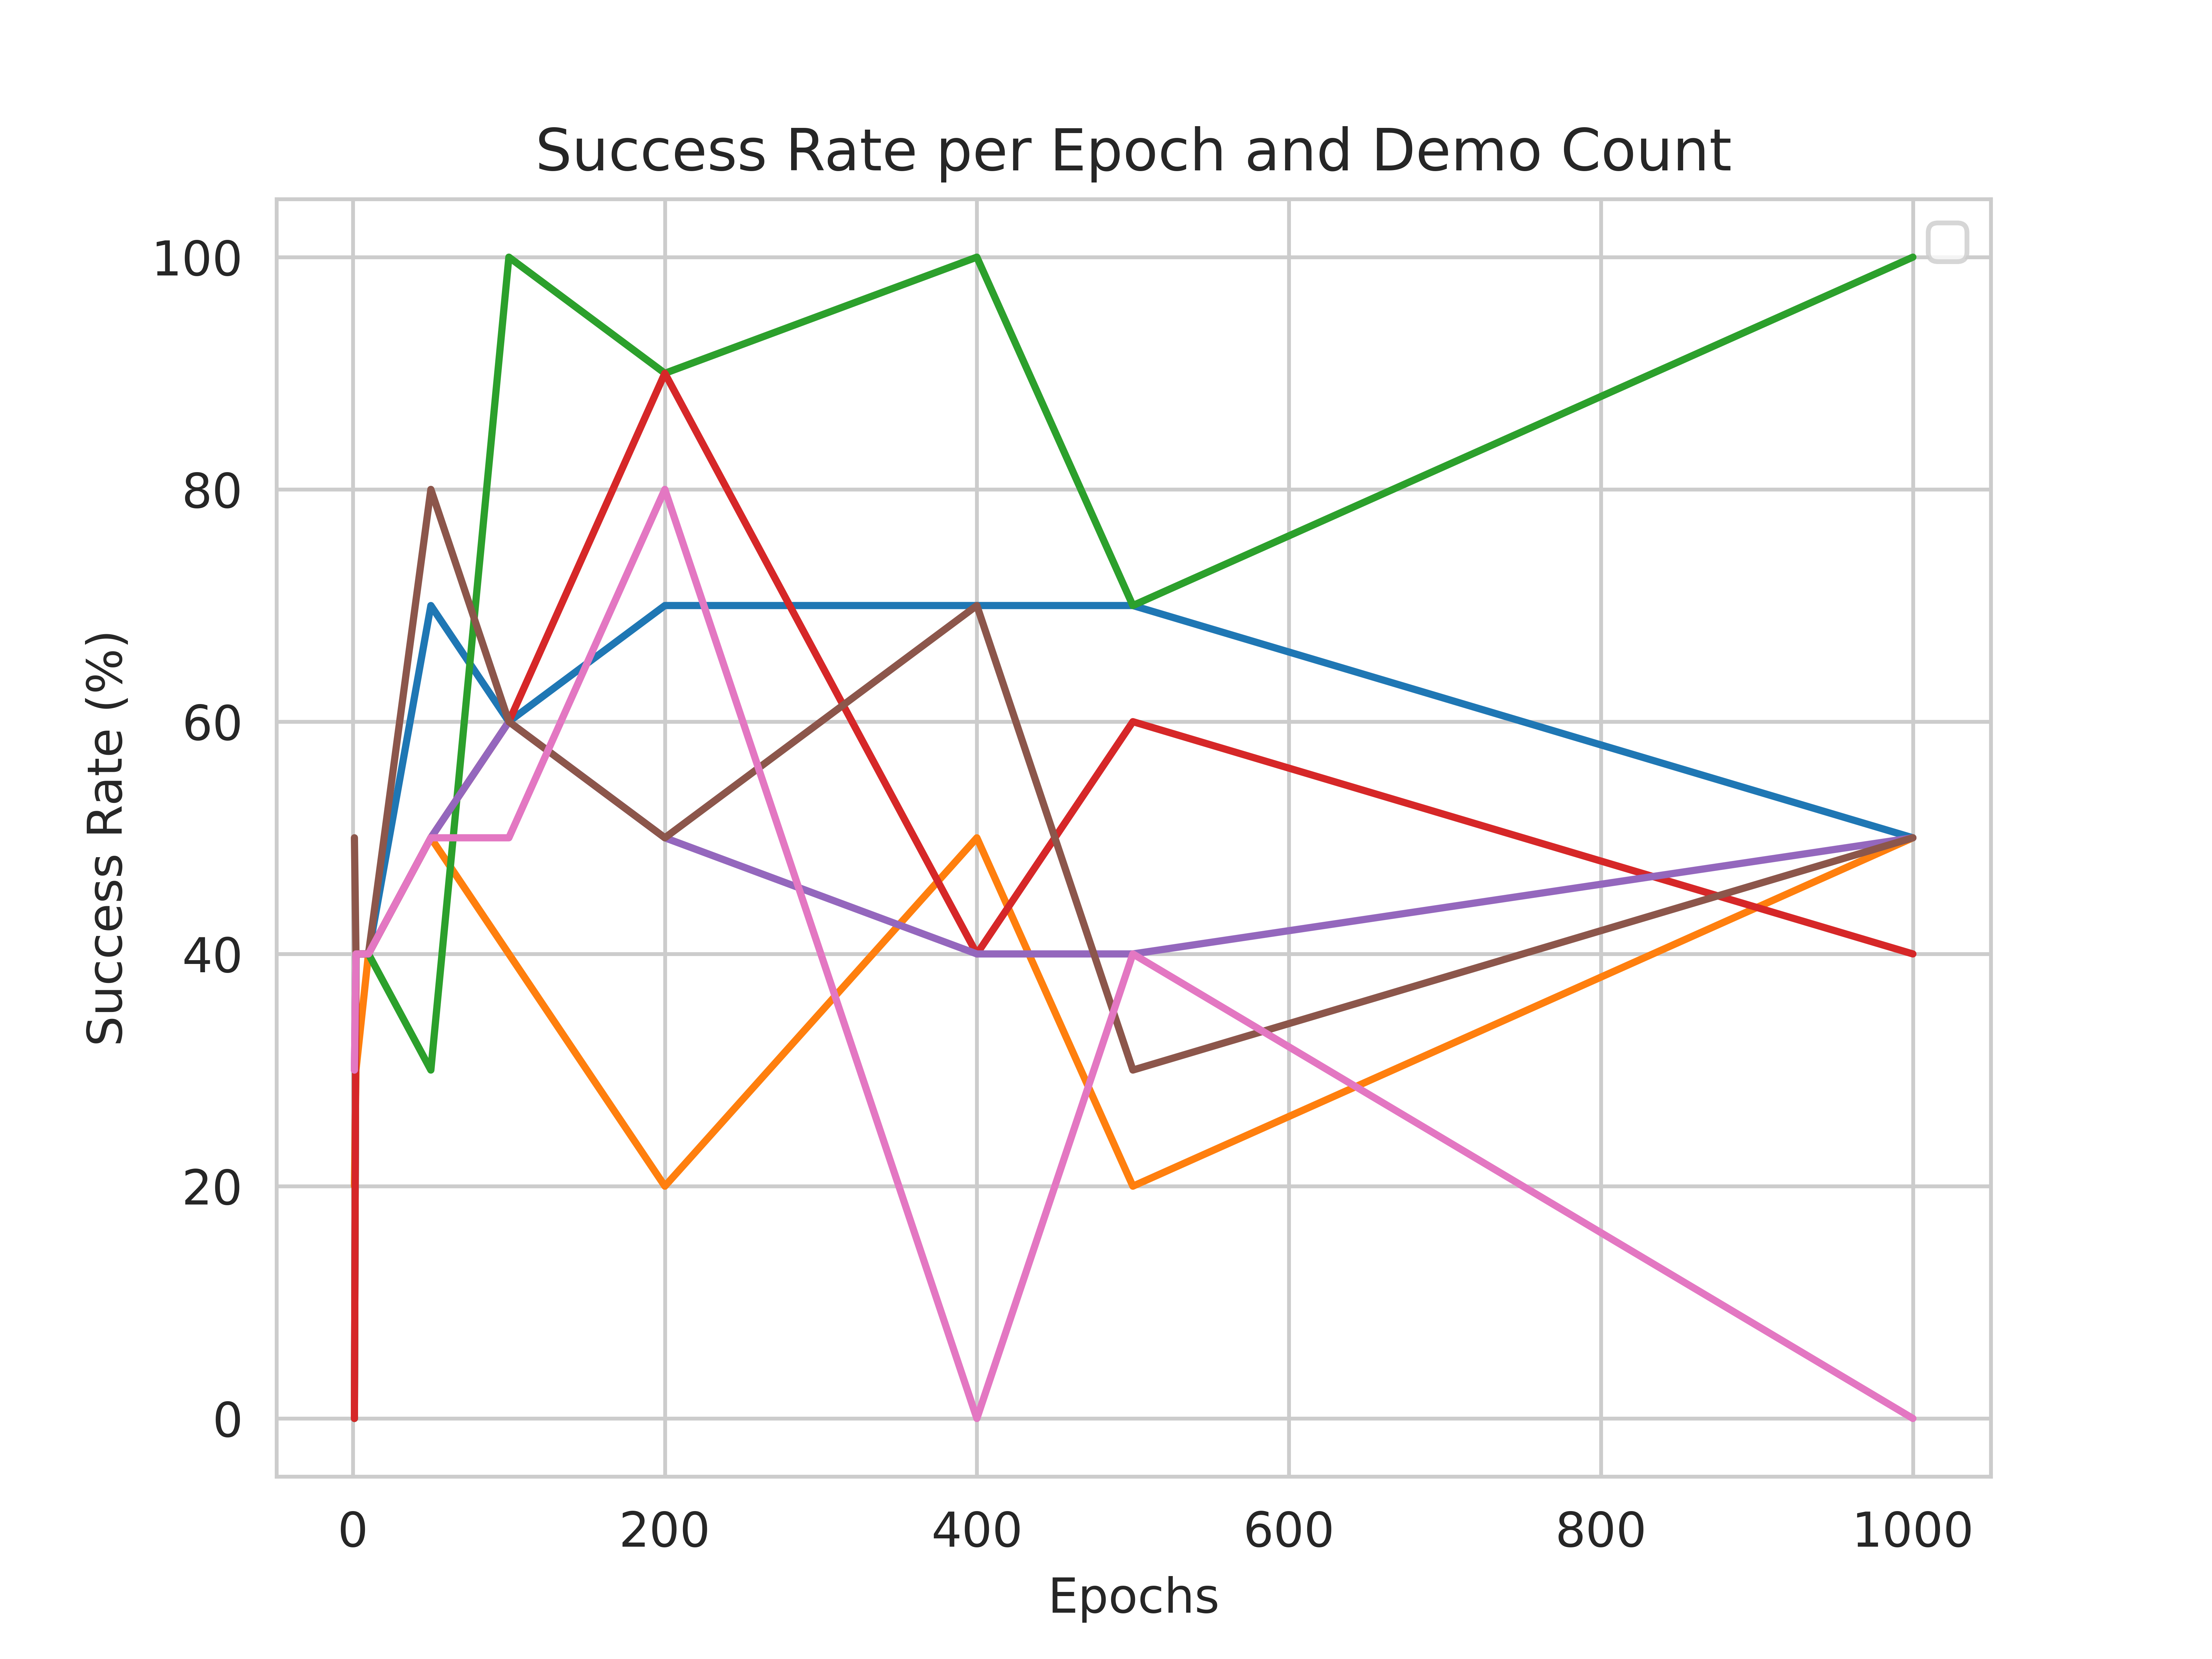
\includegraphics[width=\linewidth]{assets/cam-comb/reach-no-obs/rno_random-cam_success.png}
    \caption{Success Rate (\%) of the $10$ Demos}\label{subfig:rno-random-cams-success}
  \end{subfigure}
  \caption{Experimenting with multiple RGB cameras}\label{fig:rno-random-cams}
\end{figure}

Although the performance does not outright increase, we can clearly see that having a different point of view can sometimes drastically affect the quality of the learnt network and hence the action produced. \todo[color=purple]{}  \todo{need to actually talk about the numbers here refer to graph, talk about why the right shoulder is just better, why l and r together are lackluster}

However, this is not to say all tasks will be immune to benefits from extra views. An important part of this project is to understand what is most important for a robot to observe in its given environment and task and how can it optimally leverage this data to solve a task better. And increasingly more complex tasks should benefit from abundance of information.

\subsection{Increasing the Toy Task Complexity}\todo{subsection to above?}
Complexity of tasks can be increased in two main ways:
\begin{enumerate}
  \item Increase the movement or the level of interaction of the task at hand
  \item Introducing non-linearities to the environment to make a scene more challenging to traverse for an agent
\end{enumerate}
I plan to do these mainly by introducing obstacles; which will guide me to understand what an agent needs to understand navigation. Secondly, I want to branch out to a grasping task, to increase the number of items of execution, to evaluate the capability of an agent to use its understanding to complete increasingly more complicated tasks.\todo[color=green]{clean up depending on the chosen order}

